\chapter{Controller Development}

\section{Active Compliance}
Active vs. Passive Compliance
\section{Dynamic Stability}
Static vs. Dynamic Stability

\section{Mechanical Impedance}
Inherent mechanical impedance in the form of friction, slack, inertia, mass.

\section{Control Loop Sampling Frequency}

Limited by motor driver response time...

\Cref{fig:virtual-model-impedance-loop} is an adaptation of the control loop design found in \cite{Kalouche2016}. Continuous position loop gain scheduling vs virtual spring-damper gain scheduling.

\begin{figure}
\centering
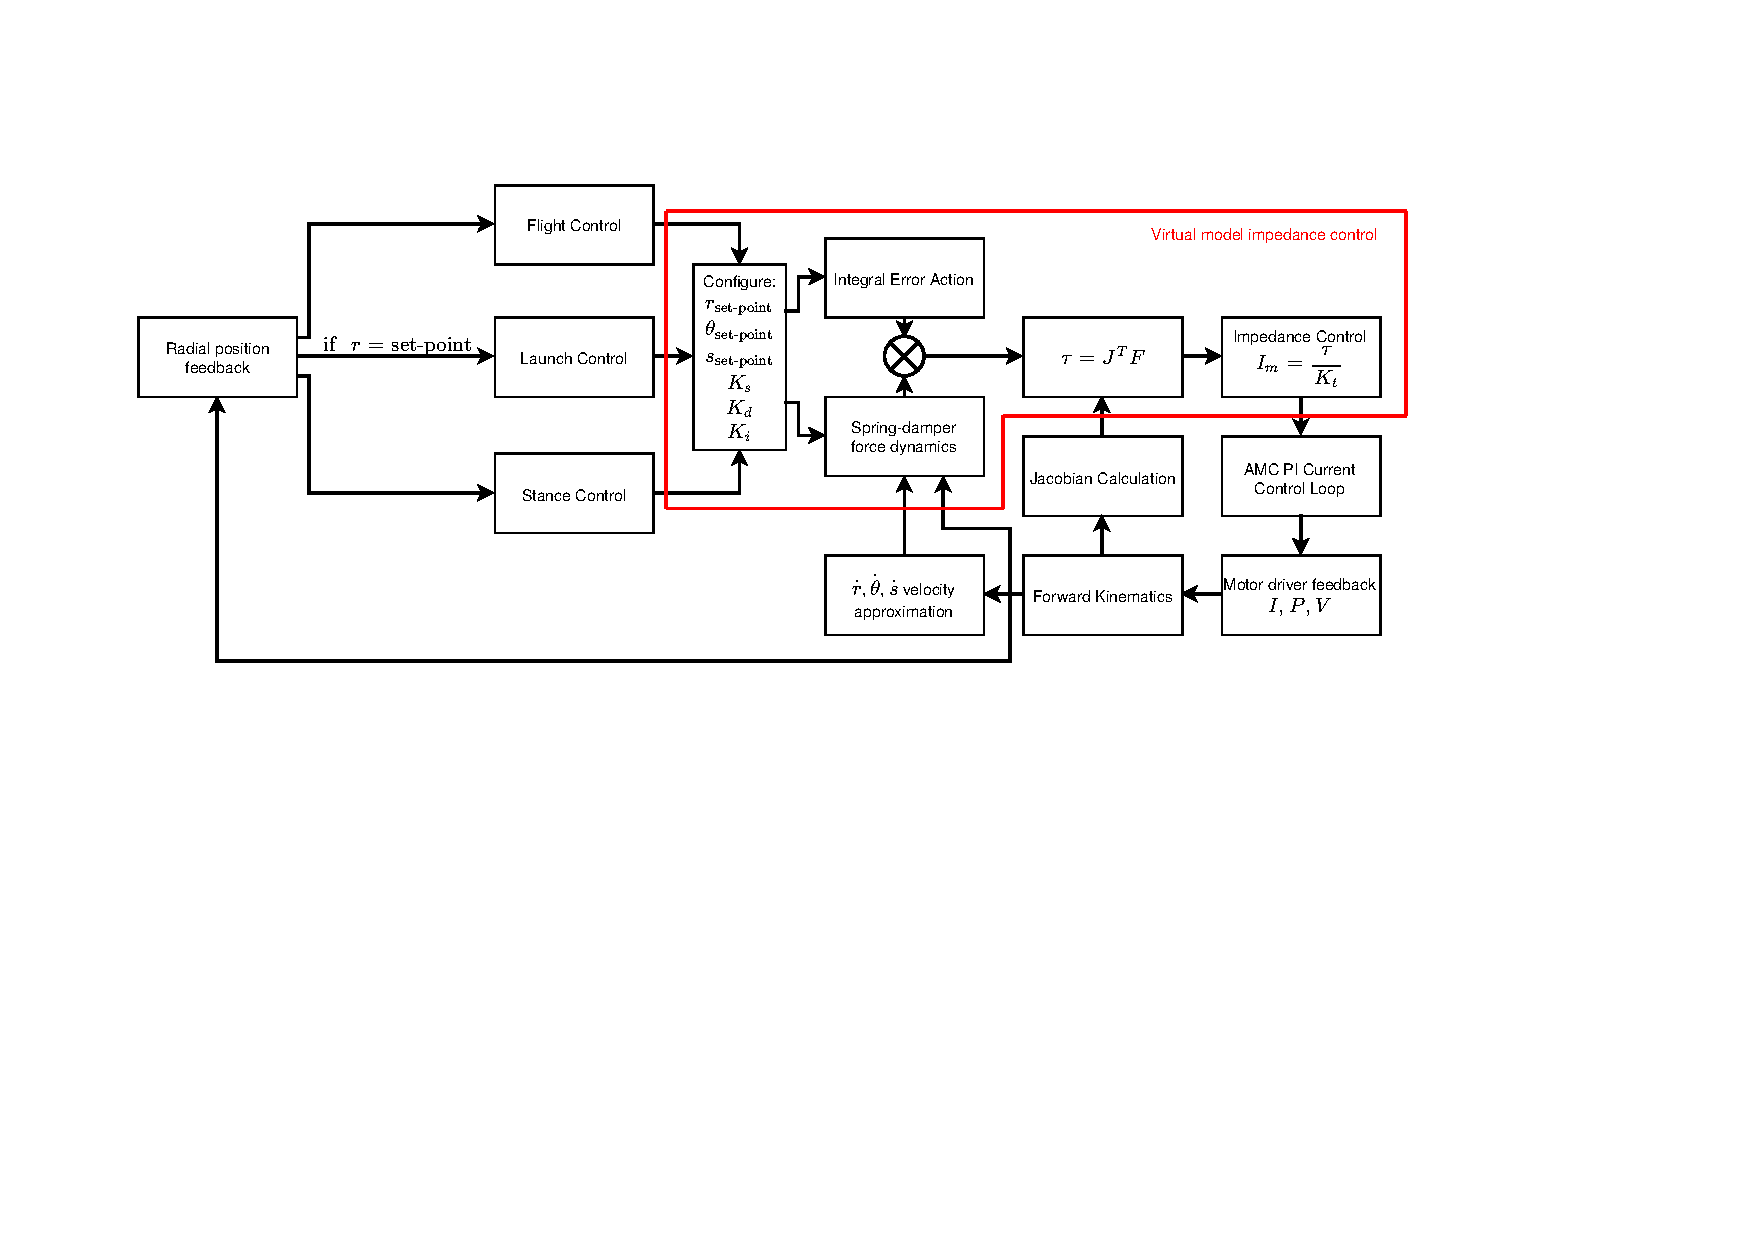
\includegraphics[clip, trim=2cm 7cm 5cm 3cm, page = 1, width=1\textwidth]{images/control/virtual-model-impedance.pdf} 
\caption{Virtual model impedance control loop.}
\label{fig:virtual-model-impedance-loop}
\end{figure}

\section{Current Control for Impulse Launch}

Current saturation at 60A.
